\chapter{Hierarchical Approximate Convex Decomposition}\label{sec:hacd}
Hierarchical approximate convex decomposition (HACD) can be used to decompose
concave objects into a collection of convex objects. These objects can be used
to simulate the scene instead.
\section{Implementation}
Bullet 2.83 contains a
composite (or compound) shape, a shape container which contains sub-shapes and acts
as a joint rigid body. Bullet updates the inertia of the object internally as
more sub-shapes are added, as well as the bounding box needed for the Sweep-And-Prune (SAP).

An implementation of HACD is included with Bullet's source code and the code is
developed by Mamou, based on the work of~\cite{mamou}. Some input parameters are available. These have been
left as the recommended parameters. The parameters control for instance concavity
penalty weights, (i.e if it is possible to disregard a small concavity)
and the maximum amount of points per convex hull.
While effective in terms of convex decomposition, this method is not particularly
effective in terms of performance. For instance, a Utah Teapot of around 4300 vertices
takes approximately 25 seconds to decompose, see figure~\ref{fig:hacdTeapot} for the result. In addition, the method is rotationally
 variant, so results may vary depending on the rotation of the object which is to be decomposed.

 \begin{figure}[H]\label{fig:hacdTeapot}
   \centering
   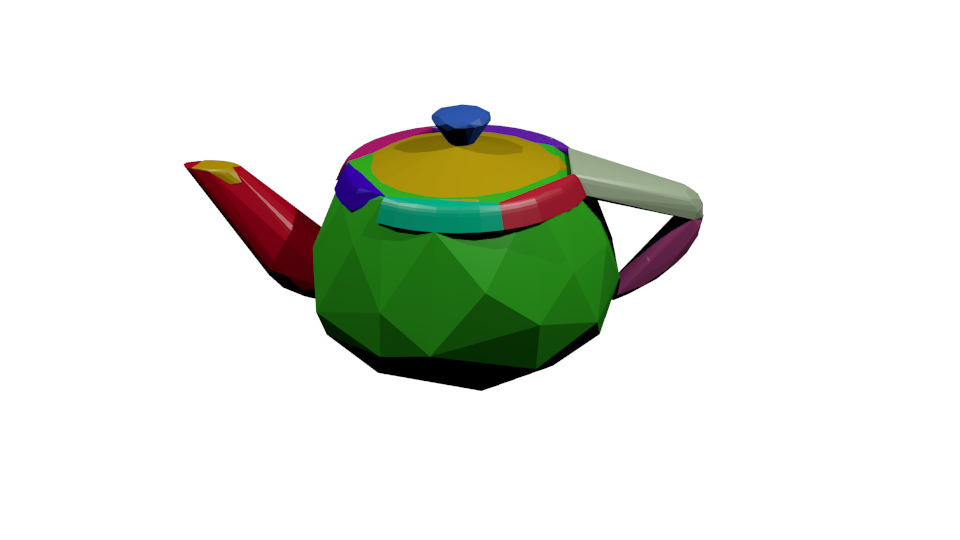
\includegraphics[width = 0.8\textwidth]{hacdTeapot.png}
   \caption{The decomposition from HACD method, model left in initial orientation}
   \label{fig:HACD}
 \end{figure}

The models are added in a three dimensional grid above the bin before the simulation
is started. Figure~\ref{fig:hacdStart} shows the start position.

\begin{figure}[H]
  \centering
  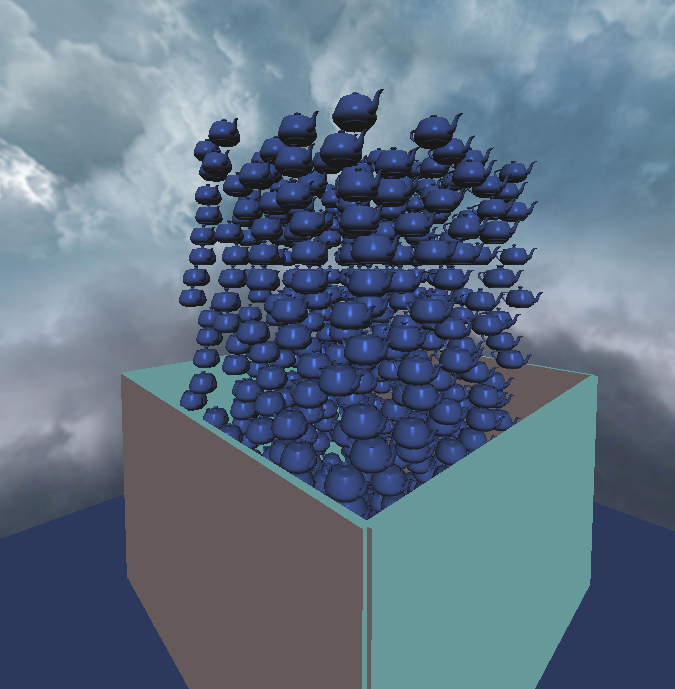
\includegraphics[width = 0.8\textwidth]{HACDstart05-11.png}
  \caption{The inital state of the simulation}
  \label{fig:hacdStart}
\end{figure}

During a simulation, much more time is spent in the last
part of the simulation when most of the models are quite stationary and only small
changes are made. The increased frametime in the later parts of the simulation is
due to the many contacts between the objects. A lot of small, rolling motions, likely due to the round
shape of the Utah Teapot, can be observed. Without the small rolling effect, Bullet's
sleeping would take effect earlier and increase performance. One can expect that
more rectangular objects will have better performance.

The result of the simulation can be seen in figure~\ref{fig:hacd0.0} and~\ref{fig:tight}.
\begin{figure}[H]
  \centering
  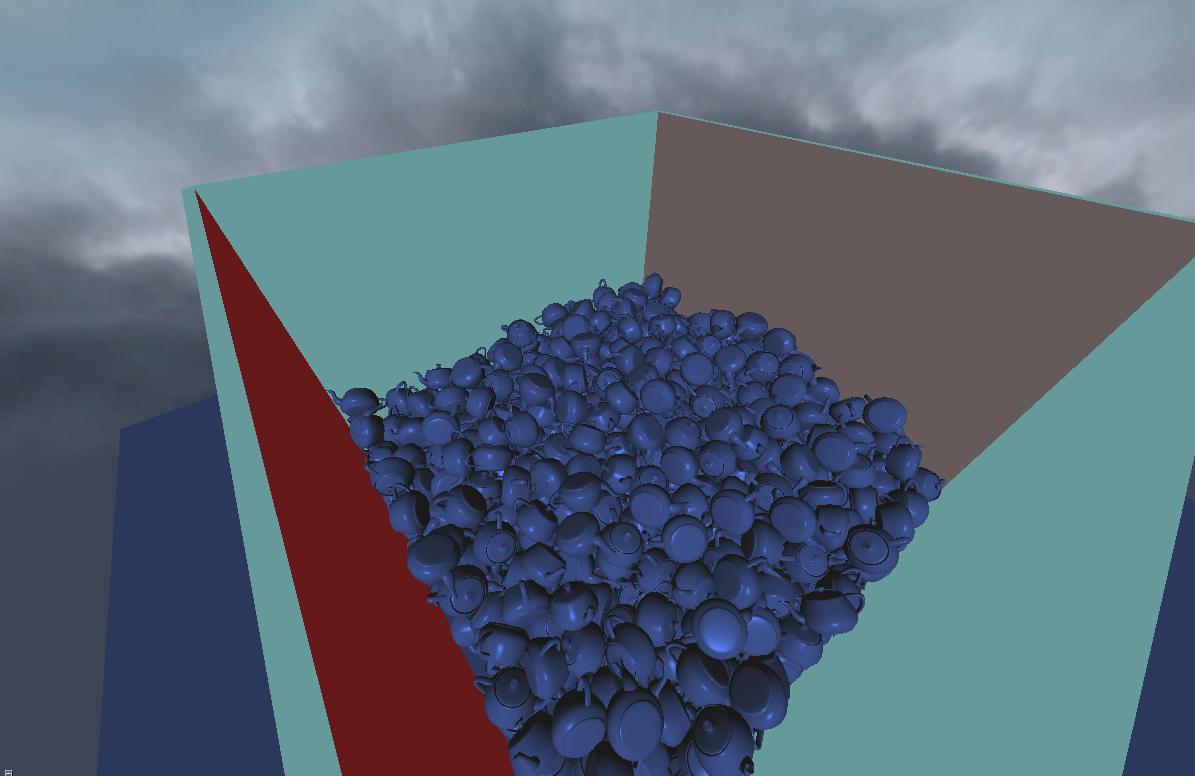
\includegraphics[width = 0.8\textwidth]{HACD512-05-11.png}
  \caption{The end result of the simulation}
  \label{fig:hacd0.0}
\end{figure}

\begin{figure}[H]
  \centering
  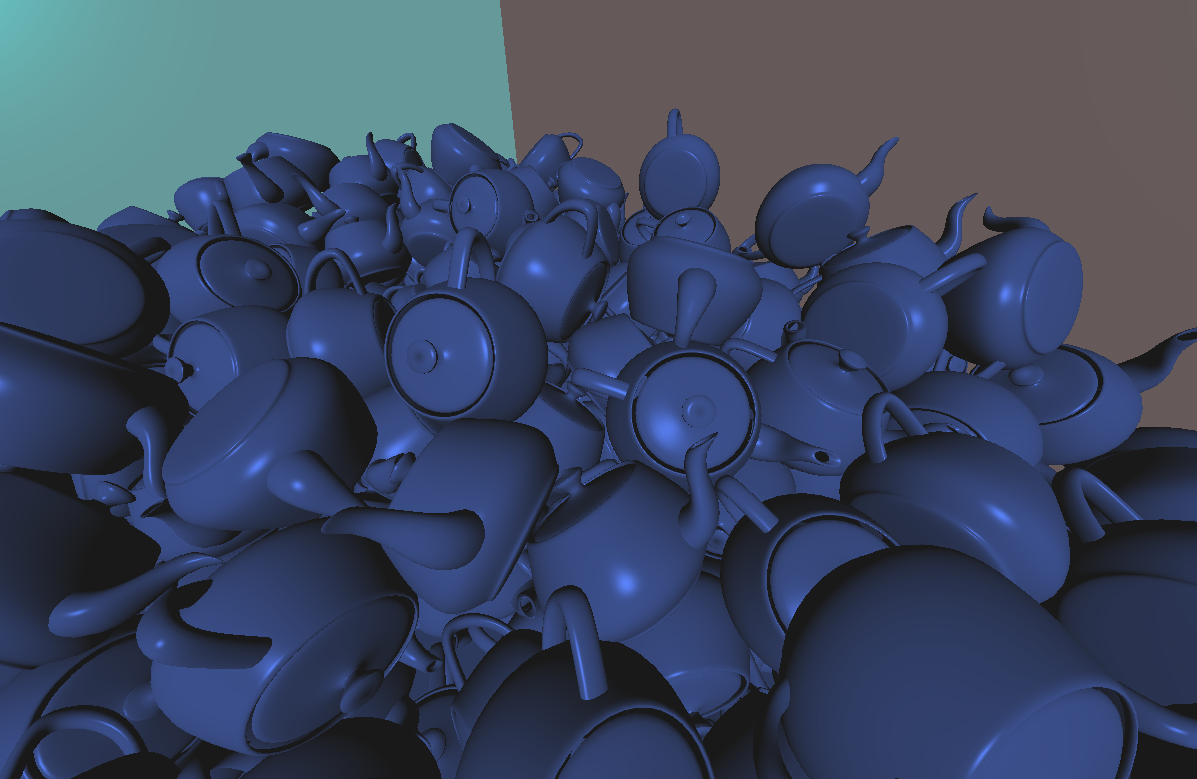
\includegraphics[width = 0.8\textwidth]{HACDtight.png}
  \caption{Close-up of final result}
  \label{fig:tight}
\end{figure}

\section{Performance}
For testing, Utah teapots consisting of twelve submodels were used. Each submodel has
between 50 and 100 vertices. A timestep of 0.01 seconds was used. All timings
presented are without rendering. All tests measure simulation
time and average the result across 2000 iterations. For the first test, Bullets' sleeping was
disabled, and for the second, the sleeping was left enabled. The results are presented
in table~\ref{tab:hacdtest}.

\begin{table}[htbp]
\caption{Testing of Bullet with HACD}
\begin{center}
\begin{tabular}{|l|r|l|}
\hline
\textbf{Sleeping Enabled} & \multicolumn{1}{l|}{\textbf{Number of objects}} & \textbf{Time/frame [ms]} \\ \hline
No & 1024 & 94.665 \\ \hline
Yes  & 1024 & 78.317 \\ \hline
No & 512 & 51.9156 \\ \hline
Yes  & 512 & 30.5515 \\ \hline
No & 256 & 22.3175 \\ \hline
Yes  & 256 & 13.298 \\ \hline
\end{tabular}
\end{center}
\label{tab:hacdtest}
\end{table}


% \begin{table}[htbp]
% \caption{Testing of Bullet with HACD}
% \begin{center}
% \begin{tabular}{|r|l|r|l|}
% \hline
% \multicolumn{1}{|l|}{\textbf{Bullet HACD test}} & \textbf{Sleeping Enabled} & \multicolumn{1}{l|}{\textbf{Number of objects}} & \textbf{Time/frame [ms]} \\ \hline
% 1 & No & 1024 & 94.665 \\ \hline
% 2 & Yes  & 1024 & 78.317 \\ \hline
% 3 & No & 512 & 51.9156 \\ \hline
% 4 & Yes  & 512 & 30.5515 \\ \hline
% 5 & No & 256 & 22.3175 \\ \hline
% 6 & Yes  & 256 & 13.298 \\ \hline
% \end{tabular}
% \end{center}
% \label{tab:hacdtest}
% \end{table}



\section{Remarks}
While the time necessary for the decomposition renders it implausible for online uses,
it is still an excellent tool for a preprocessing step.
The models can be
decomposed at the start and copies of the same shape can be used, i.e. a single decomposition
at the start of the program. For this thesis the results were also saved to an Wavefront Object (.obj) file so that simple and quick
 loading of the decomposed models could be used while testing, i.e. a single decomposition was performed and the results reused, even if the program
 was restarted.

The performance of the whole system simulation, while not phenomenal, is fast enough
for the generation of synthetic data, assuming that suitable simulation parameters
are selected.

The method does handle concave results through the approximate decomposition.

In terms of accuracy the approximate decomposition, while good, does not reproduce the objects
with perfect accuracy.

%A concave collision result is portrayed in figure~\ref{fig:concaveHACD}.

\section{Limitations}
The limitations of this method mainly concern performance. The fact
that the parameters of the HACD might affect the decomposition makes the system
on the whole less robust.
